\documentclass[a4paper]{article}
\usepackage[spanish]{babel}
\usepackage[utf8]{inputenc}
\usepackage{charter}   % tipografia
\usepackage{graphicx}
\usepackage{enumerate}
\usepackage{listings}
\usepackage{color}
%\usepackage{indentfirst}
\usepackage{fancyhdr}
\usepackage{verbatim}
\usepackage{latexsym}
\usepackage{lastpage}
\usepackage[colorlinks=true, linkcolor=black]{hyperref}
%\usepackage{makeidx}
%\usepackage{float}
\usepackage{calc}
\usepackage{amsthm, amssymb}
\usepackage[nosumlimits]{amsmath} % este package hace que se vean mal los incides en las sumatorias, pero permite poner uno abajo del otro en la ecuacon de los L de laagrange

\usepackage{subfig}

\usepackage{amsfonts}
\definecolor{gray}{gray}{0.5}
\definecolor{light-gray}{gray}{0.95}
\definecolor{orange}{rgb}{1,0.5,0}

\usepackage{color} % para snipets de codigo coloreados
\usepackage{fancybox}  % para el sbox de los snipets de codigo

\definecolor{litegrey}{gray}{0.94}

% \newenvironment{sidebar}{%
% 	\begin{Sbox}\begin{minipage}{.85\textwidth}}%
% 	{\end{minipage}\end{Sbox}%
% 		\begin{center}\setlength{\fboxsep}{6pt}%
% 		\shadowbox{\TheSbox}\end{center}}
% \newenvironment{warning}{%
% 	\begin{Sbox}\begin{minipage}{.85\textwidth}\sffamily\lite\small\RaggedRight}%
% 	{\end{minipage}\end{Sbox}%
% 		\begin{center}\setlength{\fboxsep}{6pt}%
% 		\colorbox{litegrey}{\TheSbox}\end{center}}

\newenvironment{codesnippet}{%
	\begin{Sbox}\begin{minipage}{\textwidth}\sffamily\small}%
	{\end{minipage}\end{Sbox}%
		\begin{center}%
		\colorbox{litegrey}{\TheSbox}\end{center}}



\usepackage{fancyhdr}
\pagestyle{fancy}

%\renewcommand{\chaptermark}[1]{\markboth{#1}{}}
\renewcommand{\sectionmark}[1]{\markright{\thesection\ - #1}}

\fancyhf{}

\fancyhead[LO]{Sección \rightmark} % \thesection\ 
\fancyfoot[LO]{\small{Germán Pinzón, Angel More}}
\fancyfoot[RO]{\thepage}
\renewcommand{\headrulewidth}{0.5pt}
\renewcommand{\footrulewidth}{0.5pt}
\setlength{\hoffset}{-0.8in}
\setlength{\textwidth}{16cm}
%\setlength{\hoffset}{-1.1cm}
%\setlength{\textwidth}{16cm}
\setlength{\headsep}{0.5cm}
\setlength{\textheight}{25cm}
\setlength{\voffset}{-0.7in}
\setlength{\headwidth}{\textwidth}
\setlength{\headheight}{13.1pt}

\renewcommand{\baselinestretch}{1.1}  % line spacing


\usepackage{underscore}
\usepackage{caratulaV}
\usepackage{url}
\usepackage{float}

\usepackage{underscore}
\usepackage{alltt}
\usepackage{tikz}
\usepackage{color}
\usepackage{verbatim}
\usepackage{algorithm}
\usepackage{algpseudocode}

\definecolor{dkgreen}{rgb}{0,0.6,0}
\definecolor{gray}{rgb}{0.5,0.5,0.5}
\definecolor{mauve}{rgb}{0.58,0,0.82}

\lstset{frame=tb,
  language=Python,
  aboveskip=3mm,
  belowskip=3mm,
  showstringspaces=false,
  columns=flexible,
  basicstyle={\small\ttfamily},
  keywordstyle=\color{blue},
  commentstyle=\color{dkgreen},
  stringstyle=\color{mauve},
  breaklines=true,
  breakatwhitespace=true,
  tabsize=3,
  numbers=left,
  xleftmargin=2em,
  frame=single,
  framexleftmargin=2em,
  numbersep=5pt,                   % how far the line-numbers are from the code
  numberstyle=\small\color{gray} % the style that is used for the line-numbers
 }

\parskip = 5 pt

\newcounter{row}
\newcounter{col}

\newcommand\setrow[3]{
	\setcounter{col}{1}
	\foreach \n in {#1, #2, #3} {
	\edef\x{\value{col} - 0.5}
	\edef\y{3.5 - \value{row}}
	\node[anchor=center] at (\x, \y) {\n};
	\stepcounter{col}
	}
	\stepcounter{row}
}



\newcommand\setrowaux[7]{
	\setcounter{col}{1}
	\foreach \n in {#1, #2, #3, #4, #5, #6, #7} {
	\edef\x{\value{col} - 0.5}
	\edef\y{7.5 - \value{row}}
	\node[anchor=center] at (\x, \y) {\n};
	\stepcounter{col}
	}
	\stepcounter{row}
}

\newcommand\setrowauxx[4]{
	\setcounter{col}{1}
	\foreach \n in {#1, #2, #3, #4} {
	\edef\x{\value{col} - 0.5}
	\edef\y{4.5 - \value{row}}
	\node[anchor=center] at (\x, \y) {\n};
	\stepcounter{col}
	}
	\stepcounter{row}
}


\begin{document}


\parskip = 5 pt
\thispagestyle{empty}
\materia{Organización del computador 2}
\titulo{Trabajo Práctico Final}
\subtitulo{Renderizado 3D por software}
\integrante{Germán Pinzón}{475/13}{pinzon.german.94@gmail.com}
\integrante{Angel More}{931/12}{angel_21_fer@hotmail.com}
\maketitle
\begin{abstract}
El propósito de este trabajo es desarrollar un renderizador 3D sin la ayuda de las librerías gráficas (Direct3D y OpenGL) que, junto con la placa de video, facilitan la tarea de dibujar primitivas tridimensionales. De esta manera, podemos ver que tan performante puede ser realizar este tipo de cómputos pura y exclusivamente con la CPU. El desarrollo será principalmente en lenguaje C y para las partes críticas de cálculo utilizaremos Assembler junto con SIMD para poder equilibrar un poco el hecho de no apoyarnos en la placa de video. Además, debido a que necesitamos de alguna manera dibujar píxeles en la pantalla, haremos uso de una librería gráfica de bajo nivel llamada SDL que nos permite realizar este tipo de tareas usando exclusivamente la CPU.
\end{abstract}



\newpage
\tableofcontents
\thispagestyle{empty}

\newpage
\section{Introducción}
\subsection{¿Qué es un renderizador 3D?}
Para dibujar los gráficos 3D que vemos en muchos de los juegos o software de simulación que podemos encontrar hoy en día, se hacen uso de librerías que facilitan este trabajo. En general siempre existe una abstracción de alto nivel que nos permite dibujar en pantalla un modelo o primitiva 3D de manera directa, indicando su posición en el espacio, rotación o demás características. Sin embargo, si empezamos a bajar el nivel de abstracción, siempre vamos a converger en el uso de dos librerías de bajo nivel: Direct3D y OpenGL.
\par Direct3D y OpenGL son librerías gráficas que trabajan con la placa de video independientemente del fabricante, permitiendo de esta manera que el desarrollador pueda concentrarse en el código de más alto nivel y no tenga que preocuparse por los detalles de hardware. Además, brindan el soporte matemático necesario para que el programador no tenga que realizar ciertos cálculos o construir matrices desde 0, si no que con algunos datos (por ejemplo para construir una matriz de rotación basta con pasarle el ángulo de rotación) ya se encarga de realizar la tarea por completo. De esta manera, si se desea dibujar una primitiva 3D, basta con pasar sus vértices a alguna función específica que provean estas librerías.
\par Podemos pensar entonces a un renderizador 3D como un software que se encarga de hacer ésto último, es decir, tomar la información necesaria sobre un modelo 3D (en un formato tridimensional) y convertirla a píxeles para posteriormente dibujarlos en la pantalla. Cuando decimos ``información necesaria'' estamos resumiendo muchísimas cosas ya que para dibujar un modelo 3D necesitamos bastantes más datos que solo sus vértices. El objetivo de este trabajo va a ser programar una suerte de DirectX u OpenGL propio pero que interaccione solamente con el CPU.

\subsection{Librería SDL}
SDL es una librería gráfica open source de bajo nivel, multiplataforma, que trabaja con C y que brinda soporte para el desarrollo de aplicaciones gráficas 2D (aunque puede ser usada también con OpenGL). Esta librería nos permite realizar tareas como crear la ventana, imprimir texto en pantalla, detectar eventos de mouse y teclado y pintar píxeles en la ventana de manera sencilla.
\par Elegimos SDL básicamente por dos motivos, el primero porque es una librería ``madura'' en el sentido de que lleva varios años en desarrollo y tiene una comunidad importante detras. El segundo motivo fue que también nos permite trabajar con la CPU en el sentido de que podemos evitar la aceleración por hardware de la placa de video, pudiendo de esta manera medir de manera más exacta la performance a la hora de realizar experimentos y poder sacar conclusiones más objetivamente. 

\subsection{Otras features}
Si bien nuestro principal objetivo es el de realizar los cálculos algebraicos necesarios para convertir los vértices de un modelo 3D en píxeles y así poder dibujarlos en la pantalla, existen otras cosas como por ejemplo computar transformaciones básicas sobre el objeto como rotarlo y estirarlo en distintas direcciones, aplicarle texturas y también un tipo específico de iluminación. Además, dado que en general los modelos 3D son generados por programas de diseño como 3D Studio Max o Blender y existen numerosos formatos de archivos de modelos 3D, resulta conveniente elegir uno e implementar un lector para poder cargar la información fácilmente. Nosotros elegimos el formato *.obj e implementamos dicho lector.

\section{Código SDL}
Como dijimos anteriormente, para realizar este proyecto nos apoyamos en la librería SDL y por lo tanto una parte importante del código hace uso de la misma. En esta sección vamos a detallar y explicar cuándo y para qué llamamos a la SDL.
\subsection{Inicialización, terminación y manejo de errores}
Antes de empezar a utilizar SDL hay que hacer una llamada a $SDL\_Init$ y pasarle como parámetro $SDL\_INIT\_VIDEO$ para indicarle que queremos hacer uso del subsistema de video. Esto se debe a que existen otros subsistemas de SDL como por ejemplo el que brinda soporte para el sonido. Así como debemos inicializar la librería, también debemos llamar a $SDL\_Quit$ una vez que terminamos de hacer uso de la misma (en nuestro caso antes de que el programa termine).
\par Existen numerosas funciones de SDL, algunas devuelven punteros a instancias de estructuras propias de la librería (como veremos en las siguientes secciones) y otras simplemente algún número. Es importante saber que estas funciones pueden fallar, en general las que devuelven un número, si este número es negativo significa que falló. En los casos que devuelven un puntero, fallan cuando el puntero es nulo. Para poder detectar correctamente e informar cuando una de estas funciones falla, tenemos la función $SDL\_GetError$ que nos devuelve un mensaje informándonos sobre la falla.
\subsection{Manejo de ventana}
La función SDL_CreateWindow nos permite crear la ventana donde se van a dibujar las primitivas. Dicha función devuelve un puntero a la estructura $SDL\_Window$ y nos permite definir las dimensiones y el título que queramos. Antes de terminar, el programa debe llamar a $SDL\_DestroyWindow$ y pasarle como parámetro el puntero obtenido por $SDL\_CreateWindow$.
\par En SDL para poder dibujar sobre la ventana, es necesario trabajar sobre superficies, definidas con la estructura $SDL\_Surface$. Así como cuando uno carga una imagen trabaja con la superficie asociada a la imagen, cuando queremos dibujar sobre la ventana debemos obtener la superficie asociada a la ventana utilizando la función $SDL\_GetWindowSurface$. Esta función toma como parámetro un puntero a una instancia de $SDL\_Window$ (el que obtenemos al crear la ventana) y nos devuelve el puntero a la instancia de $SDL\_Surface$ que necesitamos.
\subsection{Ciclo principal y detección de eventos}
Dado que esta es una aplicación interactiva, en el sentido de que no se trata de un software al cual ejecutamos, devuelve una entrada y termina, es necesario que todo el tiempo se esté ejecutando cierto código y ciertas llamadas a funciones. Para esto definimos un ciclo principal que termine únicamente cuando el usuario cierra la ventana. \par El ciclo principal es básicamente el nucleo de la aplicación y su condición de corte es que el usuario quiera cerrar la ventana (más adelante veremos como detectar esto). Ahí es donde se ejecuta desde la detección de eventos hasta las llamadas a las funciones encargadas de renderizar los modelos 3D, el cálculo de los FPS y otras cosas más. Cuando dibujamos un modelo 3D y decidimos rotarlo, estirarlo o cambiar el modo del renderizado debemos volver a dibujarlo todo desde cero. Para lograr esto sin que se pise con el dibujo que estaba antes lo que hay que hacer es limpiar la ventana, es decir borrar todo lo que habíamos hecho antes. De esto se encarga la función $SDL\_FillRect$, a la cuál le pasamos como parámetros el puntero a la superficie asociada a la ventana y el color que queremos que tengan todos los píxeles (para esto usamos $SDL\_MapRGB$). Luego de dibujar sobre la superficie asociada a la ventana debemos actualizarla, esto lo hacemos con SDL_UpdateWindowSurface pasándole como parámetro dicha superficie (el puntero).
\par Para el manejo de eventos primero necesitamos crear una instancia $e$ de tipo $SDL\_Event$. Luego, para detectar eventos del usuario con SDL hay que definir un subciclo del ciclo principal, cuya condición de corte es $SDL\_PollEvent(\&e) == NULL$. Si entramos al ciclo significa que detectamos un evento, para identificar que tipo de evento es usamos el campo $type$ de $SDL\_Event$ (el valor puede ser $SDL\_QUIT$ si el usuario quiere cerrar la ventana, $SDL\_KEYUP$ si el usuario soltó una tecla, $SDL\_KEYDOWN$ si el usuario está apretando una tecla, entre otros). Es cuestión de anidar distintos switches para poder identificar los eventos que nos importan y actuar en consecuencia. Dado que la detección de eventos es una parte importante del código, está toda dentro de la función $EventDetection$, la cual se ejecuta una vez por cada iteración del ciclo principal.

\subsection{Renderizado de texto (HAY QUE LLAMAR A TTF_QUIT)}
Tanto para mostrar los FPS como las indicaciones de uso, nuestro programa muestra un texto a la izquierda. Para hacer esto utilizamos una librería llamada $SDL\_TTF$ ya que SDL no brinda soporte de manera directa para renderizado de texto.
\par Esta librería es muy simple de usar y si bien es externa a SDL, está hecha para interactuar con ésta última. De manera similar a SDL, para utilizarla debemos inicializarla llamando a la función $TTF\_Init$ y antes de terminar el programa hay que hacer una llamada a $TTF\_Quit$.
\par Para empezar a hacer uso de la librería y dibujar texto en la ventana primero hay que cargar una fuente, esto lo hacemos utilizando la función $TTF\_OpenFont$ a la cual le pasamos como parámetros la ruta de la fuente que queremos utilizar y el tamaño de letra y nos devuelve un puntero a una instancia de tipo $TTF\_Font$. Una vez hecho esto ya estamos en condición de dibujar texto en la ventana, para lo cual hacemos uso de las funciones $TTF\_RenderText\_Solid$, $SDL\_BlitSurface$ y $SDL\_FreeSurface$. La primera de las tres es la que nos devuelve la superficie asociada al texto que queremos dibujar, toma la fuente que cargamos anteriormente, la cadena de caracteres correspondiente al texto y el color. La segunda función es la que efectivamente, haciendo uso de los conceptos de superficies de SDL, dibuja el texto que se encuentra en la superficie que obtuvimos con la función anterior dentro de la superficie correspondiente a la ventana. Con lo cual sus parámetros son la superficie del texto, la de la ventana y la posición (con el formato de la estructura $SDL\_Rect$). Finalmente debemos llamar a $SDL\_FreeSurface$ pasándole como parámetro la superficie asociada al texto para liberar la misma, ya que no la vamos a necesitar.
\par Como todo el proceso descripto en el párrafo anterior sobre como se dibuja texto con estas librerías puede ser un poco tedioso si lo que queremos hacer es escribir varias lineas, lo que decidimos hacer fue definir dos funciones que nos abstraigan de todos estos detalles. Estas funciones se llaman $RenderText$ y $RenderTextR$ y se encuentran definidas en sdlHelper.c. La diferencia entre ambas es que la primera no pide la posición del texto a renderizar (siempre lo dibuja arriba a la izquierda, es útil cuando solo se quiere renderizar pocos datos como por ejemplo los FPS) y la segunda sí. Ambas piden el color, la superficie asociada a la ventana, el texto y la fuente a utilizar.

\subsection{Timers}
Para medir la performance de la aplicación una de las técnicas que usamos fue el uso de timers. Si bien SDL provee soporte para esto, decidimos utilizar los clásicos Clocks de C pero hicimos uso de la función $SDL\_GetTicks$ que nos devuelve la cantidad de milisegundos que pasaron desde que se inicializó la librería.

\subsection{Función $putpixel$} \label{putpixel}
Si bien esta función no se encuentra dentro de la SDL, tiene una relación muy cercana a la misma ya que trabaja a un nivel bastante bajo con sus estructuras y formatos (efectuando operaciones como shifteos y and's) y es por eso que se encuentra en sdlHelper.c.
Toma como parámetros la superficie ($SDL\_Surface*$) de la ventana, coordenadas enteras x, y, z, un píxel en formato entero de 32 bits, tamaños enteros ancho y alto de la ventana y un puntero al depthBuffer ($float*$). Lo que hace es manipular la superficie de la ventana de manera tal de modificar el píxel que se encuentra en la posición $(x, y)$ para que ahora tenga el valor del píxel que toma como parámetro. 
\par Sin embargo, vemos que también hay otros parámetros como una coordenada z y un depthBuffer. Esto es porque, debido a que estamos renderizando en una ventana 2D que representa a un mundo 3D, cada píxel tiene una ``profundidad'' (que guardamos en el depthBuffer) y que utilizamos para testear si el píxel original que se encuentra en dichas coordenadas está delante o detras (en términos de la coordenada z) del que toma esta función por parámetro.
En el caso de que el nuevo píxel esté delante del viejo, entonces efectivamente lo modificamos, caso contrario dejamos
 todo como está.
 
\section{Implementación de estructuras}
Dado que este proyecto está realizado en C y algunas partes específicas en Assembler, no contamos con estructuras dinámicas implementadas que podamos usar de manera práctica. Estas estructuras en nuestro caso son arreglos dinámicos, las definimos nosotros en structHelper.h y sus implementaciones están en structHelper.c. Fueron construidas para el almacenamiento dinámico de coordenadas 1D, 2D, 3D y 4D a la hora de cargar un modelo 3D desde un archivo.
\par Existen varias implementaciones de estas estructuras y todas son similares, lo que cambia son las dimensiones de los puntos que almacena y el tipo de dato utilizado. Esto se debe a que a la hora de cargar un modelo 3D se necesitan cargar muchos datos de distinta naturaleza como por ejemplo los vértices del mismo (tres coordenadas de tipo float), las coordenadas de la textura en el caso de que use alguna (dos coordenadas de tipo float), los índices de los vértices (enteros) y las caras de los triángulos (tres coordenadas enteras).
\par Si observamos el código en structHelper.h, vemos que cada estructura posee una declaración similar y existen exactamente tres funciones para su manejo: la inicialización, la inserción y la liberación de memoria. Estas tres funciones nos dan el suporte suficiente para la carga de datos.
 
\section{Conceptos matemáticos}

En esta sección vamos a exponer un poco los conceptos matemáticos subyacentes de la aplicación. Las librerías gráficas que brindan soporte 3D de alto nivel como también las de bajo nivel como Direct3D y OpenGL, tratan de abstraer un poco al programador de estos conceptos. Esto significa que muchas veces el programador no necesita saber que formato tiene una matriz específica si no que simplemente llama a la función encargada de construir dicha matriz que la librería provee y listo. En este trabajo, dado que no hacemos uso de ninguna librería que brinde el soporte matemático para el manejo 3D, tuvimos que ponernos un poco más en contacto con varios de los conceptos básicos necesarios para tratar con modelos 3D y vamos a introducirlos un poco en esta sección.

\par Cuando un modelo 3D es creado, éste vive en un espacio de coordenadas por defecto (proporcionado generalmente por el programa que se utilizó para diseñarlo), conocido como espacio del modelo o $Model Space$. Luego, para poder ser renderizado pasa por múltiples transformaciones que lo llevan a otros espacios de coordenadas hasta que finalmente es visible en la pantalla. 
\par La idea se basa en utilizar tres matrices fundamentales conocidas como World, View y Projection y combinarlas utilizando el producto de matrices en una sola: 
PVW = Projection*View*World
De esta manera  multiplicando cada coordenada del objeto (en $Model Space$) por la PVW, el objeto se mueve a través de varios espacios para finalmente proyectarse en pantalla.

\textbf{Interpolación:}


Un concepto que usaremos sera el principio de interpolación lineal,  el cual nos permite obtener un tercer punto interpolado ($x_c$, $y_c$),  ajustándose a los valores de otros dos ($x_a, y_a$) y ($x_b, y_b$). Básicamente consiste en trazar una recta que pasa por ($x_a,y_a$) y ($x_b,y_b$), y calcular los valores intermedios sobre esta recta. La formula para obtenerlos es la siguiente:

$y_c$ = $y_a$ + $(x_c - x_a)*\frac{y_b - y_a}{x_b - x_c}$  (1)

Observemos que en la formula (1) $\frac{y_b - y_a}{x_b - x_c}$ es el valor de la  pendiente entre estos dos puntos es decir, la recta sobre la cual se ubicara el punto a interpolar. 
\par Dado que la formula (1) nos permite obtener el valor y del punto a polarizar a partir del x, en caso de ser conocido el valor y, y desconocido el de x si despejamos de (1) obtenemos la siguiente formula :

$x_c$ = $x_a$ + $(x_b - x_a)*gradient$ 

con $gradient$  = $\frac{y_c - y_a}{y_b - y_a}$

 
\subsection{Matriz del mundo (World Matrix)}
La primera matriz que describiremos sera la  World Matrix o Matriz del mundo.
Como mencionamos anteriormente, cada modelo vive inicialmente en un espacio local,  por lo que transformaremos sus vértices a un sistema de coordenadas común conocido como espacio de mundo o World Space. Esta matriz nos va a permitir determinar una posición,  orientación e incluso escalar el modelo en el nuevo espacio 3D.
\par La World Matrix la conseguiremos por medio del producto de otras 3 matrices, cada una de tamaño 4x4 y asumiendo una notación donde las filas representan cada uno de los ejes. Es decir la primera, segunda y tercer fila corresponden a los ejes x, y, z respectivamente y la cuarta fila se utilizará por cuestiones más matemáticas y para diferenciar entre vectores (direcciones) y puntos. Dado que adoptamos esta convención, al efectuar el producto entre un vector y una matriz, el vector deberá ubicarse a la izquierda de la matriz.
\par La $World Matrix$ se compone a su vez por distintos tipos de matrices combinadas, expresando esta combinación como el producto de estas matrices al igual que hicimos con la matriz PVW. A continuación vemos los distintos tipos de matrices que pueden utilizarse para conformar la $World Matrix$.


\textbf{Matriz de traslación (Translation Matrix)}: nos permite trasladar las coordenadas del modelo en el espacio   
 \[
\begin{bmatrix}
1 & 0 & 0 & 0 \\
0 & 1 & 0 & 0 \\
0 & 0 & 1 & 0 \\
Traslacion.x & Traslacion.y & traslacion.z & 1  
\end{bmatrix}
\]


Si bien para representar  coordenadas en un espacio 3D son necesarios tres valores (ubicación en el eje x, y y z) utilizaremos un cuarto, w, con valor 1, necesario para la aritmética matricial. En este caso Traslación indica en cuanto queremos mover cada una de las coordenadas. Traslacion.x indicara cuanto moveremos el valor x;  Traslacion.y el valor de la coordenada en y y finalmente Traslacion.z a z.
\par Si quisieramos trasladar las coordenadas (5,5,5,1) 12 unidades en dirección del eje x, al multiplicar dicho vector por la matriz de traslación obtendremos como resultado (5 + 12, 5 5, 1 ) efectivamente obteniendo el resultado deseado.  

\textbf{Matriz de escala (Scale Matrix)}: nos permite estirar en distintas direcciones al modelo
 
\[
\begin{bmatrix}
sx & 0 & 0 & 0 \\
0 & sy & 0 & 0 \\
0 & 0 & sz & 0 \\
0 & 0 & 0 & 1  
\end{bmatrix}
\]
sx, sy y sz representan el tamaño a escalar en la dirección correspondiente a la fila de la matriz. Si tomamos por ejemplo la primera fila, que representa al eje x, se puede observar que el eje conserva la dirección pero es escalado por un valor sx. 



\textbf{Matriz de rotación (Rotation Matrix )}:


 Aquí nos encontramos con distintas variantes 
 
 
 
Matriz de rotación alrededor del eje x: nos permite rotar en cierto ángulo al modelo en una dirección particular
\[
\begin{bmatrix}
1 & 0 & 0 & 0 \\
0 & cos(ang) & sin(ang) & 0 \\
0 & -sin(ang) & cos(ang) & 0 \\
0 & 0 & 0 & 1  
\end{bmatrix}
\]
Matriz de rotación alrededor del eje y:
\[
\begin{bmatrix}
cos(ang) & 0 & -sin(ang) & 0 \\
0 & 1 & 0 & 0 \\
sin(ang) & 0 & cos(ang) & 0 \\
0 & 0 & 0 & 1  
\end{bmatrix}
\]
Matriz de rotación alrededor del eje z:
\[
\begin{bmatrix}
cos(ang) & -sin(ang) & 0 & 0 \\
sin(ang) & cos(ang) & 0 & 0 \\
0 & 0 & 1 & 0 \\
0 & 0 & 0 & 1  
\end{bmatrix}
\]


Las  matrices representan  la rotación de ang grados del plano. Notemos el valor de la coordenada en el eje sobre el cual queremos rotar nunca cambia. Esto es lo que se espera cuando nosotros queremos rotar alrededor del eje en cuestión, ya que  la rotación es exclusivamente alrededor del eje y por lo tanto las coordenadas se mantienen constantes.

\par Ya vimos como es posible trasladar, estirar y rotar el modelo y como dijimos antes, es posible combinar cada una de estas transformaciones en una sola matriz ($World Matrix$): \newline
World Matrix = Rotation Matrix * Tanslation Matrix * Scale Matrix\newline  \newline
 Dado que el producto de matrices no es conmutativo entonces el orden el que se realice puede dar como resultado distintas transformaciones y posicionamiento del modelo final. Nosotros, por convención, adoptaremos el orden anterior.
Por ultimo la transformación de cada una de las coordenadas estará dada por: \newline

coordenadas\_transformadas = coordenadas\_originales * WorldMatrix 


\subsection{Matriz de vista (View Matrix)}
Como explicamos en la sección anterior, el primer paso para  renderizar un objeto 3D  es poner a todos los modelos en el mismo espacio, $World Space$. Para continuar con la proyección en pantalla de nuestro modelo necesitamos efectuar un nuevo cambio de coordenadas hacia otro espacio llamado $View Space$.

\par ¿Por que es necesario un nuevo espacio? Básicamente porque podríamos estar mirándolo desde cualquier dirección. La transformación consiste en cambiar el sistema de coordenadas de toda la escena a uno nuevo que represente la cámara que está visualizando el modelo (por eso también se lo llama $Camera Space$. Así, la matriz asociada a esta transformación ($View Matrix$) definirá la posición y orientación de la cámara, modificando sus valores alteramos el centro y el plano de proyección respecto al espacio del mundo. 
\begin{figure}[h!]
    \centering
    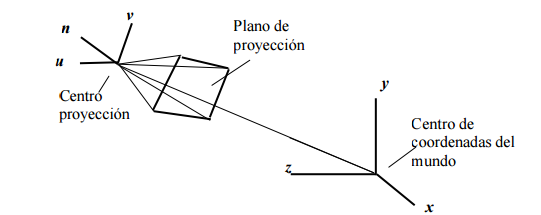
\includegraphics[width=0.50\textwidth]{Imagenes/a.png}
    \caption{Los vectores n, u, v definen los ejes principales del nuevo sistema de referencia en el $View$ $Space$.}
    \label{fig:mesh1}
\end{figure}

Para la creación de la matriz haremos uso de tres vectores $eye$, $target$ y $up$. El vector $eye$ determina la posición de la cámara con respecto al $World Space$. $target$ determina la dirección hacia donde está enfocando la cámara. $up$ que define la dirección ``hacia arriba'' desde el punto de vista de la cámara.  Una implementación típica, la cual adoptamos, es asumir que que la cámara esta colocada sobre el eje -z (left-handed coordinate system o regla de la mano izquierda por convención).
\begin{figure}[h!]
 \centering
  \subfloat[]{
   \label{f:c1}
    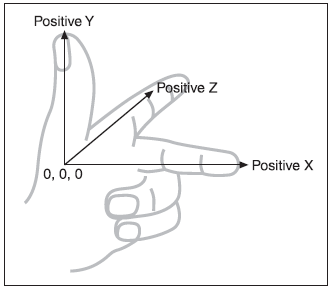
\includegraphics[width=0.4\textwidth]{Imagenes/c1.png}}
  \subfloat[]{
   \label{f:c}
    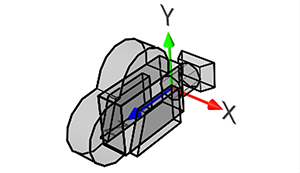
\includegraphics[width=0.4\textwidth]{Imagenes/c.png}}
  \caption{A la izquierda se muestra la ubicación de los ejes utilizando la regla de la mano izquierda y a la derecha como estaría posicionada nuestra cámara según dicha regla.}
 \label{f:coordenadas}
\end{figure}


Para construir esta matriz debemos primero calcular tres nuevos vectores: x', y' y z'. Para calcularlos vamos a empezar por z' e ir utilizando los datos que ya sabemos (como $target$, $eye$ y $up$). cross es la función que computa el producto cruzado (así aseguramos perpendicularidad) y normal la función de normalización de vectores. Así, los cálculos se efectúan de la siguiente manera: \newline \newline
    z'  = normal(eye - target); \newline 
    x' = normal(cross(up, z' )); \newline
    y' = cross(z', x');   \newline
    
    
Con estos datos podemos construir una nueva matriz que represente a estos nuevos ejes:
\[
orientation =
\begin{bmatrix}
x'.x & y'.x & z'.x & 0 \\
x'.y & y'.y & z'.y & 0 \\
x'.z & y'.z & z'.z & 0 \\
0 & 0 & 0 & 1      
\end{bmatrix} 
\]
Como la cámara todavía no está en la posición deseada ($eye$), para llegar allí se crea la siguiente matriz de traslación: \newline 
\[
translation =
\begin{bmatrix}
1 & 0 & 0 & 0 \\
0 & 1 & 0 & 0 \\ 
0 & 0 & 1 & 0 \\
-eye.x & -eye.y & -eye.z & 1 
\end{bmatrix}
\]
 Combinando la matriz de orientación con la de traslación obtendremos la matriz deseada ($View\ Matrix$):  \newline
  $View$ $Matrix$ = $orientation$ * $translation$;
  
  
Equivalentemente se puede expresar directamente como
\[
\begin{bmatrix}
x'.x & y'.x & z'.x & 0 \\ 
x'.y & y'.y & z'.y & 0 \\
x'.z & y'.z & z'.z & 0 \\
-dot(x', eye) & -dot(y', eye) & -dot(z', eye) & 1    
\end{bmatrix}
\]
Donde dot es la función que calcula el producto escalar. Este método es mas optimizado ya que no requiere realizar un producto matricial.

\subsection{Matriz de proyección (Projection Matrix)}
Todos los vértices transformados dentro del $View \ Space$ siguen teniendo tres dimensiones cuando en realidad para poder dibujarlos en pantalla se necesitan exactamente dos dimensiones. Además, aún no tenemos perspectiva, es decir, que tan lejos o cerca estamos del objeto. Dado que adoptamos la idea de posicionar la cámara sobre el eje -z, esto determinará la cercanía o lejanía con el modelo, modificando así el tamaño del mismo. La matriz de proyección será la encarga de solucionar estas cuestiones.
\par Existen distintos tipos de proyecciones, por ejemplo en una proyección en perspectiva los objetos que están más lejos de la cámara se hacen más pequeños, mientras que en una proyección ortográfica la distancia a la cámara no tiene un efecto alguno sobre el tamaño del objeto. En nuestro caso utilizaremos proyección en perspectiva.
\par La proyección en perspectiva se basa en la idea que la parte visible se encuentra dentro de una determinada figura (llamada $View \ Frustum$). El volumen de esta figura está definido por seis planos: un plano cerca de la cámara ($near \ plane$), un plano más lejos ($far \ plane$) y cuatro planos laterales que definen los bordes. El $near \ plane$  define a partir de donde se puede visualizar y el $far \ plane$ define hasta que punto podemos ver. De este modo, solo los objetos que se encuentren entre estos planos serán representados en pantalla. 
 
 
\begin{figure}[h]
    \centering
    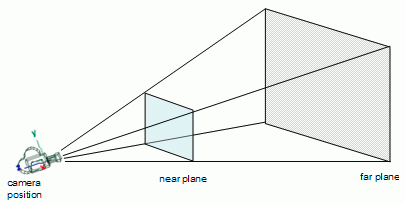
\includegraphics[width=0.50\textwidth]{Imagenes/b.png}
    \caption{Visualización basada en $View $ $Frustum$}
    \label{fig:mesh1}
\end{figure}
La matriz calculará las coordenadas dentro del intervalo [-1,1], de esta forma un punto no será visible sii luego de multiplicar la $projection matrix$ es menor que -1 o mayor que 1. Se adopta utilizar las coordenadas dentro de ese intervalo para que sea independiente de las dimensiones de la pantalla. Una vez que tengamos las coordenadas de la matriz solo deberemos multiplicarlas por el ancho y alto de la pantalla en la que se este trabajando para dimensionarlos.
\par Dado que adoptamos la ubicación de los ejes con la regla $left-handed$ estaremos posicionados sobre el eje -z. Por lo que debemos convertir cada punto de la coordenada z en -z, esto se puede lograr multiplicando las coordenadas por: 


\[
M1 =
\begin{bmatrix}
1 & 0 & 0 & 0 \\
0 & 1 & 0 & 0 \\
0 & 0 & -1 & 0 \\
0 & 0 & 0 & 1  
\end{bmatrix}
\]


De esta forma si tenemos el vector de coordenadas v = (x,y,z,1) quedaría como: \newline

v'= (x, y, -z, 1); Luego de efectuar v*M1\newline

El segundo paso requiere dividir las coordenadas x e y por -z. De esta manera cuando el objeto esté mas lejos de la cámara el valor de z sera mayor por lo que los cocientes serán más chicos (en módulo) y estaremos dándole perspectiva a nuestro objeto.
\par Recordemos que estamos trabajando con vectores de coordenadas de 4 dimensiones (conocidas como coordenadas homogéneas) donde el ultimo valor (conocido como w) es igual a 1. Si multiplicamos cualquiera de estas coordenadas por la World y/o Translation matrix observaremos que el ultimo valor se sigue manteniendo en un 1 (que es lo que queremos). Sin embargo, no es el caso cuando multiplicamos por esta matriz. Esto significa que para volver a las coordenadas homogéneas, luego de haber multiplicado el vector de coordenadas por la matriz PVW, tendremos que dividirlo por el valor w que posea ya que de esta forma estaremos efectuando $\frac{w}{w}$ obteniendo de nuevo el valor 1. Entonces, si w fuese igual a -z, conseguiríamos lo que estamos buscando: dividir x e y por -z.\newline

Consideremos cambiar la cuarta columna de la matriz M1 por el siguiente vector (0,0,-1,0) tenemos una M2 tal que:

\[
M2 =
\begin{bmatrix}
1 & 0 & 0 & 0 \\
0 & 1 & 0 & 0 \\
0 & 0 & -1 & -1 \\
0 & 0 & 0 & 0 
\end{bmatrix}
\]

De esta forma un vector v = (x, y, z, w) quedaría como (x, y, z, -z) luego de efectuar v*M2 ya que:\newline

w'=$x*0$ $+$ $y*0$ $+$ $z*(-1)$ $+$ $1*0$ $=-z$

Esto tiene por efecto establecer w como -z pero, si -z es diferente a 1, entonces tendrá que ser normalizado es decir, vamos asignar z al rango [0,1]. Para ello, vamos a utilizar los valores $near$ $plane$ y $far$ $plane$. \newline
Estableceremos los coeficientes de la matriz utilizada M2 cambiando los valores de la tercera columna por (0, 0,$\frac{-f}{f-n}$,$\frac{-f*n}{f-n}$ ), siendo $f$ el valor de $far$ $plane$ y $n$ el valor de $near$ $plane$, y veamos que sirve:\newline

Ahora tendremos la matriz:

\[
M3 =
\begin{bmatrix}
1 & 0 & 0 & 0 \\
0 & 1 & 0 & 0 \\
0 & 0 & \frac{-f}{f-n} & -1 \\
0 & 0 & \frac{-f*n}{f-n} & 0  
\end{bmatrix}
\]

Sea v = (x, y, z, w) luego de efectuar v*M3 tendremos un nuevo vector v' con la tercer coordenada igual a: 


z' =$x*0$ $+$ $y*0$ $+$ $\frac{-f}{f-n}$*$z$ + $\frac{-f*n}{f-n}$*$1$

Se deberían cumplir dos condiciones: cuando v este mas cerca del $near$ $plane$ z' debería ser 0 y mientras mas cerca de $far$ $plane$ debería tender al valor 1. 


 Veamos cuando z es igual a $-f$
 
 z'= $\frac{-f}{f-n}$*$(-f)$ + $\frac{-f*n}{f-n}$*$1$ = $\frac{f*f + -f*n}{f-n}$ = $\frac{f*(f-n)}{f-n}$ = $f$
 
 
 Y cuando z es igual a $-n$
 
 
 z'= $\frac{-f}{f-n}$*$(-n)$ + $\frac{-f*n}{f-n}$*$1$ = $\frac{f*n - f*n}{f-n}$ = $0$
 
Recordemos que aun es necesario dividir por w' que es -z por lo que en el primer caso -z = $f$ entonces, tendríamos como resultado final 1; en el segundo caso 0. Efectivamente obtuvimos los valores deseados.


Por último, hay que tener en cuenta el ángulo de visión (AOV)  o campo de visión (FOV) de la cámara. Este parámetro controla qué parte de la escena es visible a la cámara.\newline
Generalmente se utiliza es suponer que la ventana de proyección es un cuadrado de [-1: 1] en cada dimensión. y que la distancia entre la misma y la cámara es igual a 1. 


\begin{figure}[h]
    \centering
    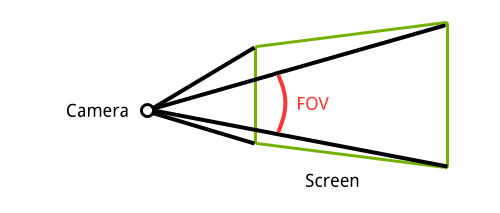
\includegraphics[width=0.50\textwidth]{Imagenes/d.png}
    \caption{Con verde la porción de la pantalla que queda delimitada al utilizar FOV.}
    \label{fig:mesh1}
\end{figure}

\pagebreak

Dado que la parte observable de nuestro mundo 3D puede variar de acuerdo al valor de FOV, debemos incluirlo de alguna manera en nuestro cambio de coordenadas. Sin entrar en detalle en la trigonometría que hay detras de esto, se utiliza el valor $P = 1 \ / \ tan(FOV * 0.5)$. Esto nos va a permitir escalar las coordenadas para poder definir la visibilidad de los vértices de acuerdo a este ángulo y no solo al posicionamiento de los mismos.
La matriz de proyección entonces queda de la siguiente forma:


\[
\begin{bmatrix}
P & 0 & 0 & 0 \\
0 & P & 0 & 0 \\
0 & 0 & \frac{-f}{f-n} & -1 \\
0 & 0 & \frac{-f*n}{f-n} & 0  
\end{bmatrix}
\]


Ya tenemos todas las matrices necesarias, con lo cual si multiplicamos cada coordenada dentro del $Model \ Space$ por la matriz PVW estaremos casi en condiciones de tener representado nuestro modelo en la pantalla. Lo único que falta es dividir estas coordenadas por $w'$ y mapear estos valores a las dimensiones de nuestra pantalla.\newline


Llamemos $x''$ e $y''$ a las coordenadas finales que permitirán graficar en nuestra pantalla al modelo 3D y ($x'$, $y'$, $z'$, $w'$) al valor obtenido luego de multiplicar una coordenada por PVW tendremos que: \newline

$x''$ = $\frac{x'}{w'}*width +  width*0.5$ \newline

$y''$ = $\frac{y'}{w'}*height +  height*0.5$ \newline

Donde $width$ y $height$ representa el ancho y alto de nuestra pantall. Notar que luego sumamos $width*0.5$ a $x''$ y $height*0.5$ a $y''$ para tener las coordenadas finales centradas en la pantalla.

\subsection{mathHelper}
En el archivo mathHelper.h declaramos numerosas funciones matemáticas que luego definimos en mathHelper.c. Estas funciones van desde cálculos básicos como el producto cruzado, el producto escalar, normalizaciones y productos de matrices hasta la construcción de matrices específicas como de rotación, escala, vista y proyección.
\par Existen cálculos que se repiten mucho a lo largo del código y que, en algunos casos, es necesario realizarlos por cada ejecución del ciclo principal por ejemplo. En estos casos decidimos implementar también una versión de los mismos en Assembler con el objetivo de optimizar la performance y poder realizar mediciones y comparaciones con las versiones de estas funciones en C. Las funciones matemáticas que decidimos implementar en Assembler son las siguientes: producto escalar (ScalarProdASM), interpolación (InterpolateASM, hablaremos del uso de esta función más adelante) y producto de vector por matriz (Vec4Mat4ProductASM). También existen otras funciones que decidimos implementar en Assembler, que no realizan cálculos matemáticos pero que se ve reflejado en la experimentación que haberlas programado en Assembler mejoró notablemente la performance, hablaremos de ellas más adelante.

\subsection{sdlHelper: }



Luego de tener las coordenadas como vectores bidimensionales procederemos a la rasterización de los mismos,  es decir trasformar los vectores de coordenadas en píxeles. Recordemos que los vértices de nuestro modelo están agrupados de  modo que forman un triángulo entre si. Elaboraremos tres modos que aplicaran distintos efectos sobre el modelo. 


\subsection{Modo 1:}



\par Inicialmente nuestro modelo esta conformado por polígonos mas específicamente triángulos. Blender nos permite obtener los vértices de los mismos por lo que el primer modo se encargara de reconstruir los polígonos.
\par Construiremos una nueva función llamada $DrawTriangle\_m1$ que sera la encargada de transformar los puntos bidimensionales proyectando y rellenando los triángulos en nuestra pantalla.

\textbf{DrawTriangle\_m1 y ProcessScanLine\_m1:}

\par  Sean v1,v2,v3 los tres vértices que forman un triangulo, la función renombrara dichos vértices como P1, P2, P3 de manera que P1 sea el que se encuentre en una posición menor o igual que P2 respecto del eje y;  P2 a su vez sera aquel que se encuentre en una posición menor o igual que P3 respecto del mismo eje. 
\par Definiremos P1.y como el valor en la coordenada y de P1, P1.x como el valor en el eje x y de manera análoga para P2, P3, SX y EX. 
\par La idea para crear las aristas es definir para cada valor Y entre P1.y y P3.y dos puntos SX y EX como se observa en la figura 5 de esta manera la sucesion de puntos creara la idea de aristas.


\begin{figure}[h]
    \centering
    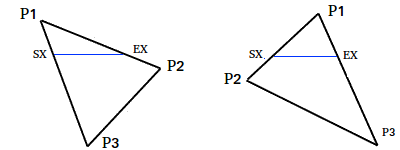
\includegraphics[width=0.50\textwidth]{Imagenes/e.png}
    \caption{Alguno de los posibles triángulos que se pueden formar con los valores del eje y aumentando hacia abajo y los del eje x hacia la derecha.}
    \label{fig:mesh1}
\end{figure}

\par La principal incógnita que se nos plantea es encontrar el valor SX.x y EX.x (ya que SX.y y EX.y es igual al valor Y de la iteración) de manera que se ubique dentro de la recta que los uniría. Para esto utilizaremos la formula de interpolación a partir de conocer el valor del eje y; mientras que los puntos que requiere la función seran los que conformen la recta sobre la cual se encuentren SX y EX.
\par La función encargada de usar la interpolación de los puntos y proceder con la creación de las lineas la denominaremos $ProcessScanLine\_m1$ quien sera llamada por $DrawTriangle\_m1$ en los diferentes escenarios que se nos planteen.


Sea pa, pb los puntos que me permiten interpolar SX y pc y pd los que interpolan a EX podemos definir: 


\begin{verbatim}
ProcessScanLine_m1(pa, pb, pc, pd, Y):
    gradient1 = if (pa.y != pb.y) 
                    (Y - pa.y) / (pb.y - pa.y)
                else 1                          
    gradient2 = if (pc[1] != pd[1]) 
                    (Y - pc.y) / (pd.y - pc.y)
                else 1;
            
    SX.x = Interpolate(pa.x, pb.x, gradient1)
    EX.x = Interpolate(pc.x, pd.x, gradient2)
    
    putpixel(SX.x, Y);
    putpixel(EX.x, Y);
\end{verbatim}


Como mencionamos $DrawTriangle\_m1$ hará uso de esta función en los distintos casos que se nos presenten, ya que si observamos la figura 5 vemos que no siempre SX o EX se encuentran sobre la misma arista, en un caso SX esta en la arista correspondiente a P1 y P3 mientras que en el otro triangulo esta sobre la conformada por P2 y P1 esto nos lleva a plantearnos y analizar todos los casos antes de comenzar el proceso de crear las lineas.


Primero estableceremos una manera de distinguir cuando P1 se encuentra a la derecha de P2 o viceversa: 

dP1P2 = (P2.x - P1.x) / (P2.y - P1.y) 

dP1P3 = (P3.x - P1.x) / (P3.y - P1.y)


Que representan las pendientes inversas de los puntos que se utilicen. Dado que el valor del eje y se incrementa hacia abajo dP1P2 sera positivo cuando P2 este a la derecha de P1 mientras que dP1P3 sera negativo, cumpliendose que dP1P2 $>$ dP1P3; y para el caso de P2 a la izquierda de P1 tenemos que dP1P2 $<$ dP1P3. \par Dado que P2.y podria ser igual a P1.y o P3.y igual a P1.y entonces asignaremos el valor cero a dP1P2 y dP1P3 correspondientemente.



Continuando con los posibles escenarios, decidimos divir los casos que se presentan cuando P2.y es distinto de P1.y y cuando es igual.\newline
\par Cuando P2.y es distinto a P1.y se nos presentan los primeros dos casos:
 
\begin{itemize}
\item Primer caso: P1 se encuentra a la derecha de P2 (dP1P2 $>$ dP1P3). Se puede observar en el triangulo izquierdo de la figura 5. SX.x se obtiene a partir de los puntos P1 y P3, en cambio EX hasta el valor P2.y puede ser calculado con P1 y P2 pero luego se utilizara a P2 y P3.

\item Segundo caso: P1 se encuentra a la izquierda de P2 (dP1P2 $<$ dP1P3). Correspondiendose al lado derecho de la figura, vemos que EX.x se obtiene a partir de P1 y P3, mientras que SX.x con P1 y P2 hasta que se llegue al valor Y $=$ P2.y y luego con P2 y P3. 

Cuando P2.y es igual a P1.y tenemos que evaluar lo siguiente:

\item Tercer caso:  SX.x se obtiene por los puntos P1 y P3 , mientras que EX.x por P2 y P3 si P1.x es menor a P2.x en caso contrario SX.x es consecuencia de P2 y P3 mientras que EX.x de P1 y P3 


\end{itemize}


Una vez planteadas las distintas situaciones podemos proceder con la rasterización de los triángulos. 
  
El código fuente que describe el proceso anterior es el siguiente:

\begin{verbatim}
DrawTriangle_m1(v1,v2, v3): (CREO QUE SE PODRIA DEJAR LA EXPLICACION DE LOS CASOS ANTERIORES 
O ESTE PSEUDOCODIGO SOLAMENTE NO SE.....)

    Designar P1, P2 y P3 
    
    Calcular dP1P2 y dP1P3
    
    if (Primer Caso)
            for (Y = P1.y to P3.y)    	
                if(Y < P2.y)
                    ProcessScanLine_m1(P1, P3, P1, P2, Y)
                else
                    ProcessScanline_m1(P1, P3, P2, P3, Y)
    if(Segundo Caso)
           for (Y = P1.y to P3.y)    	
                if(Y < P2.y)
                    ProcessScanLine_m1(P1, P2, P1, P3, Y)
           else
                    ProcessScanline_m1(P2, P3, P1, P3, Y)
    if (Tercer Caso)	
          for (Y = P1.y to P3.y)    	
               if(P1.x < P2.x)
                    ProcessScanLine_m1(P1, P3, P2, P3, Y)
               else
                    ProcessScanline_m1(P2, P3, P1, P3, Y)
  					
\end{verbatim}


\subsection{Modo Textura:} 

\par En el segundo modo procederemos a rellenar los triángulos adoptando la idea del algoritmo Scan Line. El mismo se basa en rellenar cada triangulo de izquierda a derecha por medio de un conjunto de pixels (que representaría la linea azul en la figura 5) y, continuando con la notación del modo anterior, descendiendo desde P1.y hasta P3.y.  
\par Comenzaremos sobre el punto SX ubicado sobre las aristas del lado izquierdo de los triángulos y procederemos a crear una sucesión de puntos, incrementando el valor de SX.x, hasta llegar al extremo derecho es decir, al punto EX.x. Esta idea la aplicaremos empezando a iterar desde un valor Y igual a P1.y y cada vez que se completa una linea procederemos a aumentar el valor Y para crear una nueva, hasta que llegar a P3.y. 
La técnica para rellenar los triángulos sera la definida anteriormente ahora tenemos que definir los valores que tendrán esos pixels es decir, su color y mas aun su textura (en el caso de tener la información necesaria).
Blender nos permite dentro del programa asignarles texturas a los distintos modelos, una de las formas es tomando como input una imagen y utilizando la Mapeo UV ($UV$ $mapping$). Esta técnica permite asignar una textura en 2D a una superficie 3D. 
\par A cada vértice ,de los polígonos que componen el modelo, le sera asignado un par de coordenadas 2D llamas UV. Este nuevo par de coordenadas definen que área de la imagen es mapeada a cada triangulo es decir, permitirá pintar cada triangulo con el color de una imagen. 
\par No solo podemos exportar los vértices sino que también las coordenadas UV de cada uno (si hemos pasado por el proceso de asignarle una textura previamente).
\par Como requeriremos acceder a cada píxel de la imagen usaremos la función $SDL\_LoadBMP$ ( provista por SDL) la cual permite cargar una superficie desde un archivo del tipo .BMP y nos devuelve un puntero a la misma, al cual llamaremos $tex$.    
 
\par Por lo que $DrawTriangle\_m1$ sera modificada a $DrawTriangle\_m2$ de manera que cada vez que llame a $ProcessScanLine\_m2$ (que sera una variante de $ProcessScanLine\_m1$) además pasara las coordenadas UV de los vértices utilizados y el puntero a la textura.
 
\textbf{ProcessScanLine\_m2:} 


Ahora esta función tendrá las coordenadas UV para cada vértice. En cada una de las lineas que vamos construyendo definimos dos puntos SX y EX y luego procedemos a calcular sus valores intermedios, ahora también sera necesario calcular las coordenadas UV asociadas a estos. La forma de calcularlos sera por medio de la interpolación. Si los puntos pa y pb nos permitían obtener SX y, pc y pd a EX de manera similar si utilizamos las coordenadas U asociadas a estos vértices podemos calcular un valor $su$ y $eu$ que indiquen el rango de valores que utilizaremos de la coordenada U; mientras que con las coordenadas del eje V podemos calcular $sv$ y $ev$ delimitando el rango de valores usados de V.
\par Una vez calculados $su$, $eu$ podremos interpolar los valores intermedios para calcular las coordenadas U de los puntos entre SX.x y EX.x e interpolando con $sv$ y $ev$ obtendremos los valores del eje V.
\par Dado que las coordenadas en los ejes UV están entre los valores cero y uno, una vez calculadas las coordenadas UV de cada punto sera necesario escalarlas para acceder correctamente en $tex$. Solucionaremos esto definiendo la función $map$ que realiza el producto del ancho de la imagen con el valor de la coordenada U y el producto del alto de la imagen con la coordenada V e indexara en $tex$.
Por ultimo dibujar cada punto con el color asociado estará a cargo de $Draw\_point$. En caso de no tener una textura cargada simplemente asignaremos un numero de color arbitrario.  

A partir de este modo implementaremos el uso del $depthBuffer$ mencionado en \ref{putpixel} por lo que sera necesario además interpolar el valor z asociado a cada punto para luego poder comparar y así dibujar o no un píxel.

 
\par finalmente podemos expresar la función por medio de siguiente pseudocódigo: 




\begin{verbatim}
ProcessScanLine_m2(pa, pb, pc, pd, Y, tex):
    gradient1 = if (pa.y != pb.y) 
                    (Y - pa.y) / (pb.y - pa.y)
                else 1                          
    gradient2 = if (pc[1] != pd[1]) 
                    (Y - pc.y) / (pd.y - pc.y)
                else 1;
            
    SX.x = Interpolate(pa.c, pb.c, gradient1) //.c coordenadas luego del producto por WVP
    EX.x = Interpolate(pc.c, pd.c, gradient2)
    su = Interpolate(pa.U, pb.U, gradient1) //.U denota al valor en la coodenadas U
    eu = Interpolate(pc.U, pd.U, gradient2)
    sv = Interpolate(pa.V, pb.V, gradient1).V denota al valor en la coodenadas V
    ev = Interpolate(pc.V, pd.V, gradient2)
    z1 = Interpolate(pa.z, pb.z, gradient1)
    z2 = Interpolate(pc.z, pd.z, gradient2)
   

    for (x = SX.x to EX.x)
        gradient = (x - sx) / (float)(ex - sx)
        z = Interpolate(z1, z2, gradient)
        u = Interpolate(su, eu, gradient)
        v = Interpolate(sv, ev, gradient)
        if (tex != NULL)
            textureColor = Map(tex, u, v)
        else
            textureColor = 0xfffffff;
    
        putpixel(x, Y, z, textureColor)
\end{verbatim}

\subsection{Modo Textura + Sombra:} 

	El tercer modo se basa en simular efectos de luz sobre la superficie del objeto. Para esto definiremos un punto que sera desde donde iluminaremos nuestro modelo, lo llamaremos $lightPos$. Para calcular la luminosidad nos basaremos en la técnica Gouraud Shading, la misma utiliza 3 vectores normales por cada triangulo que compone a nuestro modelo. Estos vectores serán normales pero, a los vértices de cada uno. Otros métodos utilizan solo un vector normal a la superficie de los triángulos pero de esta forma toda la superficie obtiene la misma intensidad de color en cambio la técnica que emplearemos nos permite tener variaciones de intensidad sobre una misma superficie. 
\par Como podemos iluminar a nuestro modelo desde cualquier punto del espacio donde vive nuestro modelo y no específicamente desde nuestro punto de vista, sera necesario entonces definir $lightPos$ teniendo en cuenta que se utiliza las coordenadas del World Space así también como los vectores normales (que serán exportados por Blender) y los vértices asociados. Como mencionamos, originalmente los vértices y, en este caso, las normales viven dentro del Model Space para convertirlas a World Space solo necesitaremos multiplicar por la World Matrix.   Luego de tener las coordenadas en los respectivos espacios llamaremos a la función DrawTriangle.




\textbf{DrawTriangle\_m3:} 

 	Extenderemos la versión anterior, $Drawtriangle\_m2$, de manera que ahora calcule la luz que recibe cada vértice.
\par La idea de los vectores normales es que cuanto menor sea el ángulo entre estos y la dirección de la luz (figura 6) entonces la luz incidirá más sobre el vértice asociado y de esta manera la intensidad del color se mantendrá, en caso contrario tendera a un color mas oscuro para simular sombras. 
	
	
	\begin{figure}[h]
    \centering
    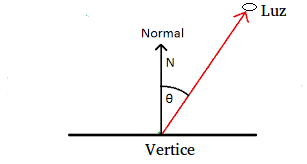
\includegraphics[width=0.50\textwidth]{Imagenes/f.png}
    \caption{}
    \label{fig:mesh1}
\end{figure}


	Dado que no tenemos el vector dirección de la luz pero si la posición y la coordenada sobre la cual incide ($centerPoint$) procederemos a calcular la dirección como:

 $lightDirection$  = $lightPos$ – $centerPoint$


	Una de las formas que podemos calcular la intensidad de luz que llega a cada vértice es con el coseno del ángulo formado por lightDirection y cada vector normal. Cuando el ángulo es cero entonces el coseno es igual a uno, lo de que denotara la idea de luminosidad máxima; si bien la función coseno tiene como imagen valores entre [-1; 1] fijaremos como valor mínimo cero que representara luminosidad nula. De esta forma podemos observar que si multiplicamos el color por 1, valor de luz máxima, se sigue manteniendo igual el color mientras que si el valor decrece el color sera mas oscuro hasta llegar  a 0 por lo que obtendremos el color negro. 
\par El coseno de un ángulo $\theta$ formado por dos vectores A y B se puede calcular como:

cos($\theta$) = $\frac{A*B}{\parallel A \parallel*\parallel B \parallel}$ 

con $\parallel A \parallel$ y $\parallel B \parallel$ la distancia Euclidiana de A y B respectivamente.

 
Si normalizamos el vector A y B el denominador  sera igual a  1 y de este manera solo calculando el producto vectorial podemos obtener el coseno del ángulo. 
Calcularemos $lightDirection$ junto con el coseno del ángulo asociado en una función auxiliar $ComputeNdotL$ que sera llamada en DrawTriangle para cada vértice, y utilizaremos estos valores para extender la función $ProcessScanLine\_m2$ en una nueva versión llamada $ProcessScanLine\_m3$.
   
\textbf{ ProcessScanLine\_m3:}

Tenemos el porcentaje de luz para las coordenadas que representan a los vértices, solo nos falta para el resto de las que componen cada triangulo,  por lo que cada vez que interpolemos las coordenadas para rellenar el triangulo, también interpolaremos la luz que recibiría  basándonos en la que tienen los vértices. Por ultimo solo debemos multiplicar este valor por el color del punto interpolado.

\section{Análisis de performance y experimentación}
En esta sección vamos a presentar varios resultados de distintos tipos de mediciones que realizamos. Observando estos datos vamos a poder explicar el porqué de la definición de algunas funciones en Assembler y otras en C que sustituyen a otras funciones originales de la aplicación que realizan un mayor consumo de cómputo.

Dado que se trata de una aplicación interactiva en el sentido de que no es el tipo de software que se ejecuta, devuelve un output y termina, realizar mediciones puede ser un poco más complicado. Lo que nosotros decidimos hacer fue poner una cota superior a la cantidad de iteraciones que realiza el ciclo principal de la aplicación (mencionado en la sección 2) ya que es el encargado de ejecutar toda la funcionalidad que se provee. Una vez que se alcanza esa cota, la aplicación termina.

Además, dado que existen varios modos de renderizado y trasnformaciones que le podemos hacer a nuestro modelo mientras la aplicación está corriendo, es necesario elegir alguna configuración posible para poder realizar las mediciones. En nuestro caso el modo de renderizado 1 (esqueleto) no lo vamos a utilizar ya que necesita muy poco poder de cómputo para poder ejecutarse, en cambio los modos 2 (con textura) y 3 (con textura y sombra) sí los vamos a usar. Además, vamos a hacer que el modelo rote en las tres direcciones (hacemos esto para aumentar la cantidad de operaciones matriciales que realiza la aplicación), con la velocidad de rotación que viene por default. No se va a realizar escalado una vez que el modelo ya esté dibujado, es decir, el modelo va a conservar el tamaño original o el que configuremos al cargarlo si es necesario aplicar un reescalado para que entre en la pantalla. El modelo que vamos a utilizar para realizar las mediciones va a ser alfred.obj, con su correspondiente textura alfred.bmp.

La herramienta gprof nos provee un informe detallado del consumo de cada una de las funciones de la aplicación. De esta manera, luego de correr gprof obtenemos, entre otras cosas, una tabla con el porcenaje de tiempo consumido por cada función. Nosotros nos vamos a concentrar en las funciones que más tiempo consumieron, ignorando así otras donde el consumo es mínimo y no nos proveen información relevante.

\subsection{Optimización del código encargado de la interpolación}
Comencemos haciendo una corrida de gprof a nuestra aplicación con el código hecho exclusivamente en C y veamos si podemos mejorar algo a partir de eso. 

\begin{figure}[h]
    \centering
    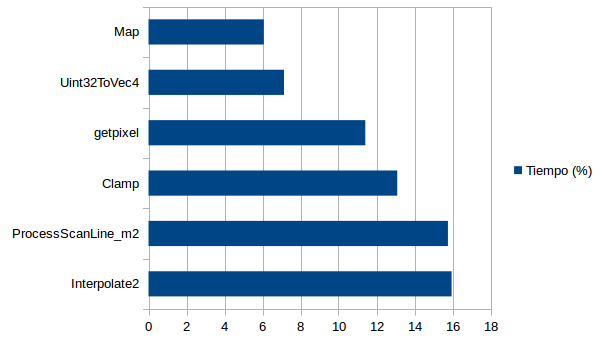
\includegraphics[width=0.8\textwidth]{Imagenes/gprof1.png}
    \caption{Código puramente en C, rotación en los tres ejes, renderizado en modo 2 y 1000 iteraciones del ciclo principal.}
    \label{fig:mesh1}
\end{figure}


Podemos ver que la función Interpolate2 es la que más consumo de tiempo realiza y le siguen ProcessScanLine_m2 y Clamp. Recordemos que tanto Interpolate2 como Clamp, son funciones matemáticas que son llamadas durante el proceso de rasterización. Más aún, Interpolate2 realiza una llamada a Clamp en su definición y a su vez ProcessScanLine_m2 llama sucesivas veces (14 para ser exactos) a Interpolate2. Claramente estas tres funciones están muy vinculadas entre sí y debido a las numerosas llamadas a Interpolate2, la idea va ser optimizar ésta función.

En cuanto a las otras funciones, Map y getpixel están muy relacionadas con SDL ya que Map lo que hace es simplemente realizar un cálculo con el ancho y el alto de una textura y ciertas coordenadas para obtener otras coordenadas (en píxeles), llamar a getpixel y devolver el valor del píxel precisado. En principio es dificil pensar una manera de optimizar esto porque además Map es llamada una sola vez (en ProcessScanLine_m2) y getpixel también (en Map). Finalmente Uint32ToVec4 hace algo bastante simple que es convertir un color en formato uint32 (con el que trabaja SDL) a vector de float que es el tipo de dato que utilizamos nosotros en nuestras funciones. Lo hace mediante ANDs, shifteos y divisiones con lo cual también se trata de una función bastante minimal en cuanto a operaciones que realiza.

Para tratar de mejorar Interpolate2 lo que vamos a hacer es que no llame a Clamp. Es decir, la función Clamp también tiene un consumo considerable y el hecho de que Interpolate2 se llama tantas veces y ésta a su vez llama a Clamp puede evitarse haciendo Clamp dentro de interpolate. Para esto, vamos a definir entonces Interpolate1 y veamos que resultados nos arroja gprof ahora:

\begin{figure}[h]
    \centering
    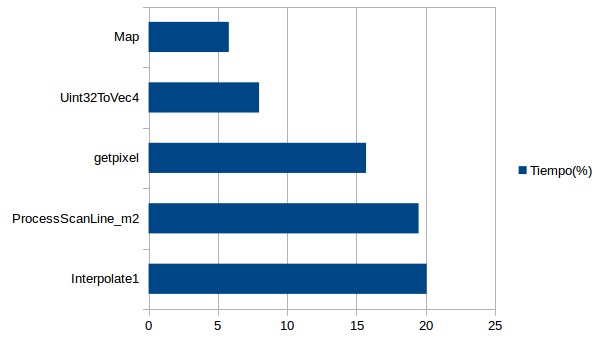
\includegraphics[width=0.8\textwidth]{Imagenes/gprof2.png}
    \caption{Misma configuración de parámetros iniciales, ahora Clamp está dentro de Interpolate1.}
    \label{fig:mesh1}
\end{figure}

Se puede ver que el porcentaje de tiempo consumido es un poco mayor en Interpolate1 que antes en Interpolate2 y lo mismo sucede con ProcessScanLine_m2. En principio, pareciera que lo que hicimos empeoró las cosas, sin embargo sucedió todo lo contrario. El porcentaje de aumento que se registró en estas funciones se debe a que gracias a que ahora no existe Clamp, el tiempo total que tarda el programa en realizar las 1000 iteraciones es menor. Dado que la cota de iteraciones no cambió, la cantidad de veces que se ejecuta cada función sigue siendo la misma y en consecuencia el porcentaje del tiempo de consumo de las funciones que quedaron aumentó.

Para corroborar este hecho observamos además que los FPS aumentaron aproximadamente el doble con Interpolate1 y el tiempo que tardó la aplicación en llegar a las 1000 iteraciones fue considerablemente menor también.

Ahora veamos que datos obtenemos renderizando en modo 3 con la misma configuración de parámetros y hagamos la comparación entre estas dos versiones de Interpolate.

\begin{figure}[H]
    \centering
    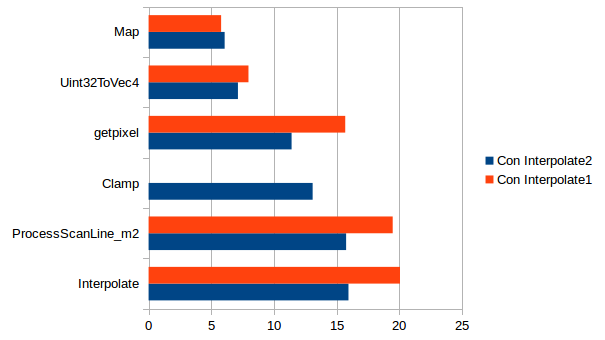
\includegraphics[width=0.8\textwidth]{Imagenes/gprof3.png}
    \caption{Misma configuración de parámetros iniciales salvo que ahora renderizamos en modo 3.}
    \label{fig:mesh1}
\end{figure}

Vemos que la comparación en este modo es muy similar a la del modo anterior. En cuanto a tiempos y FPS pasa algo similar (el tiempo disminuye y los FPS aumentan considerablemente al utilizar Interpolate1) solo que en este caso los tiempos son un poco mayores debido a que es el modo más costoso por los cálculos con las normales.

\subsection{Optimizaciones en Assembler}
Como explicamos en la sección anterior, las mediciones realizadas hasta ahora fueron hechas sobre el código en C. Decidimos implementar varias funciones en Assembler, sobre todo las que hacen procesamiento matricial pero también otras como la encargada de la interpolación y la de limpiar el depth buffer y ver si esto efectivamente representa una mejora en la performance. A continuación mostramos los resultados que arroja gprof con las funciones que venimos analizando hasta ahora.

\begin{figure}[H]
    \centering
    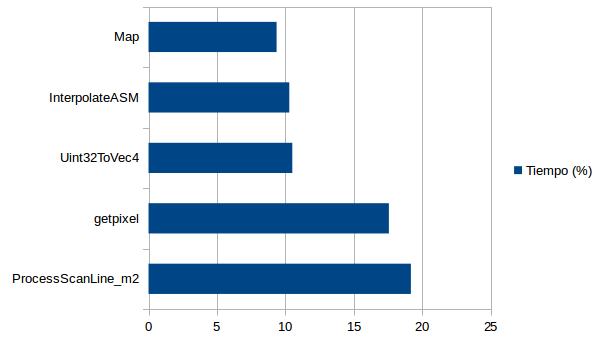
\includegraphics[width=0.8\textwidth]{Imagenes/gprof4.png}
    \caption{Misma configuración de parámetros iniciales, modo 2.}
    \label{fig:mesh1}
\end{figure}

El consumo que realiza InterpolateASM ahora es significativamente menor comparado con el que realizaba Interpolate1 e Interpolate2. Esta nueva implementación en Assembler efectivamente reduce los recursos que necesita esta función para ejecutarse.

Como dijimos antes existen otras funciones que decidimos implementar en Assembler, no podemos mostrar sus porcentajes de consumo aca porque el gprof no arroja esos resultados. Esto puede ser porque son muy pequeños (ya eran relativamente pequeños en sus versiones de C) y no los tiene en cuenta. Sin embargo, el tiempo total que tarda en ejecutar las 1000 iteraciones esta versión en Assembler es considerablemente menor, sobre todo cuando estamos en modo 3. El siguiente gráfico muestra los tiempos en segundos de cada una de las versiones con los distintos modos:

\begin{figure}[H]
    \centering
    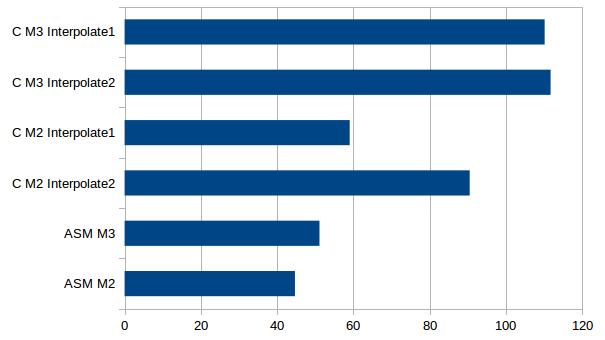
\includegraphics[width=0.8\textwidth]{Imagenes/tiemposTotales.png}
    \caption{Tiempos totales en finalizar las 1000 iteraciones con las distintas versiones. Fueron medidos en un procesador i5 con 8gb de RAM.}
    \label{fig:mesh1}
\end{figure}


\end{document}